\chapter{Assessing Shape Demonstration Correctness} \label{chap:correctness}
In a system whose main goal is to improve the handwriting of children with difficulties it is a must to be able to evaluate the progression over time for two main reasons: Providing a useful output of the child improvement to the activity supervisor and testing the efficiency of the system in the handwriting.  

\section{Motivation}
One of the main missing points in the current system is a proper metric to evaluate the demonstration provided by the user. Since people have the ability to assess intuitively when a letter is well written and when it is not, it becomes necessary to study a mathematical solution for a quantitative assessment when a child is performing an iterative task. Such outcome can be very useful for both the robot and the supervisor to adapt the behavior and to study the improvement of the children during the interaction or along several sessions, respectively. The goal of this stage of the project is to provide a suitable approach of inter-shape distance.
 
\section{Statistical shape modeling with PCA in the CoWriter}
The current system for the generation of the synthetic handwriting is based on a statistical shape modeling using Principal Component Analysis (PCA) \cite{stegmann2002brief} on the shape of the letters \cite{hood2015children}, whose basics will not be introduced in this work. 

By definition, the goal of PCA is to summarize the correlations among a set of observed variables with a smaller set of linear combinations. Because it is trying to capture the total variance in the set of variables, PCA requires that the input variables have similar scales of measurement, in our case being similar shapes. For instance, faces or samples of the same letter. But what is more important is that each component's eigenvalue represents how much variance it explains. 

In the case of the initial formulation of the CoWriter project several steps were accomplished in order to generate these shapes (the result is implemented in the \textit{shape learner\footnote{https://github.com/chili-epfl/shape\_learning}} python library). Firstly, the eigenspaces are generated over a set of letter paths captured from a digital pen and stored in a dataset (UJI Pen Characters 2) \cite{ujidataset}. Once a demonstration is provided by a child and projected to the correspondent letter eigenspace, it gets decomposed in their principal components. From this point new similar shapes can be generated by modifying the largest eigenvalues. Therefore, the robot response can be computed by modifying the eigenvalues towards midway between the child demonstration and a reference shape (a considerably good letter).

Based on the previous statements it is a must to capture as much variance as possible to properly provide similar shapes as the ones received from the user. However, this variance among same type of shapes can only be decoded if the eigenspace is able to capture it. In another words, the dataset used to build the eigenspace needs to be as rich as possible in terms of children mistakes variability. It was necessary then, to build a new dataset which includes that information, based on real children demonstrations.

Moreover, since the eigenspaces represent the main features of the letters, a good metric to compare two letters may be the Euclidean distance between their eigenvalues. For instance, in figure \ref{fig:datasets} can be observed the difference between the original dataset and the new one in terms of shape demonstration distances with respect to the reference shape. But also the difference when a new demonstration is included to the dataset for the generation of a new eigenspace (dynamic) or when it is not (static). In the case of the dynamic one, since after each demonstration shape the eigenspace is recomputed, we expect that the new eigenspace is able to capture more variance leading to greater distances between the demonstrations and the reference shape.

\begin{figure}[h!]
        \centering
        \begin{subfigure}{0.9\textwidth}
                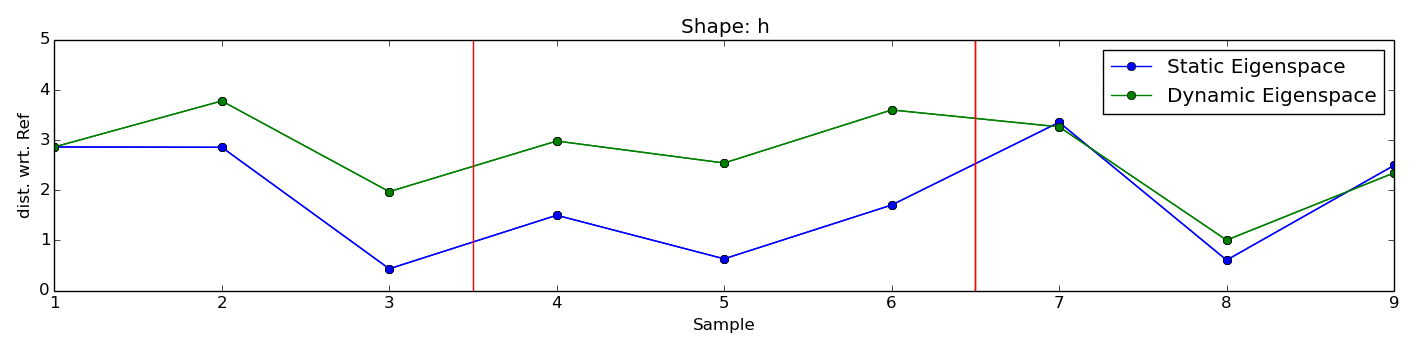
\includegraphics[width=1\textwidth]{figures/uji_pen.png}
                \caption{Uji pen dataset}
                \label{fig:ujipen}
        \end{subfigure}%

        \begin{subfigure}{0.9\textwidth}
                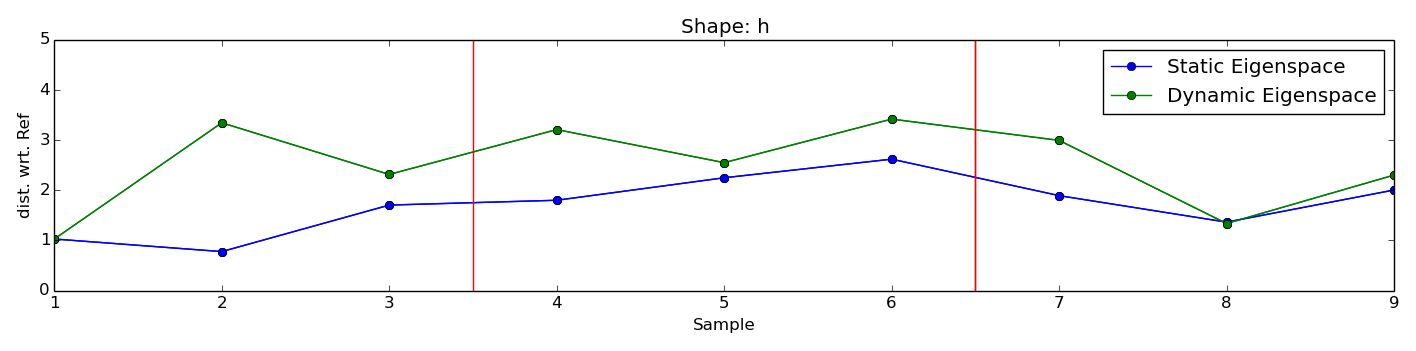
\includegraphics[width=1\textwidth]{figures/alexi.png}
                \caption{New dataset}
                \label{fig:alexi}
        \end{subfigure}
        \caption{Euclidean distance between the demonstration shapes and the reference shape in the eigenspace generated by the two datasets with (dynamic) and without (static) demonstration addition across different sessions (red lines)}
        \label{fig:datasets}
\end{figure}

In the case of \textit{uji pen} dataset (figure \ref{fig:ujipen}) we can see how in each iteration the distances of the demonstrations with respect to the reference shape has a higher variability in comparison with the \textit{new dataset} (figure \ref{fig:alexi}) which shows smoothed values (see blue lines). The reason is due to the greater variance captured by the second one. 
Furthermore, the distance between the demonstrations projected to a dynamic (green lines) and the ones projected to a static eigenspace (blue lines) remains smaller with the new dataset, getting reduced after certain amount of iterations. It suggests that the previous demonstrations did not induce a greater variance in the new eigenspace whereas in the old one did. Such results are provided using an Euclidean distance as metric. However, it is still remaining to be understood which metric can be more suitable to assess distances in the eigenspace in a reliable way. Examples would be City block distance or Mahalanobis distance among others.

\section{Uniform point distribution}  

From the acquisition of a user's demonstration till the generation of a shape response from the system, several steps were already implemented in the \textit{shape learner} library. Indeed, the shape generation pipeline has been improved in later revisions of the initial version. Currently, it includes several preprocessing steps before a shape is projected to the correspondent eigenspace and their values used for the shape generation. In figure \ref{fig:shapeProcess} the contribution of this section has been highlighted in the pipeline. 

\begin{figure}[h!]
        \centering
        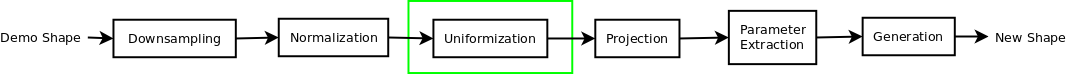
\includegraphics[width=1\textwidth]{figures/shapeProcess.png}
        \caption{Shape generation pipeline }
        \label{fig:shapeProcess}
\end{figure}

The current implementation of the system allows to capture the user input from the tablet in order to be processed and generate a similar shape in response. However, such points collected in the tablet need to be down-sampled to be independent from the time the tablet stylus remained on the screen surface. All shapes then, are reduced to 70 points using a cubic interpolation of a 1-D function.

In this way, it is necessary to normalize the shapes to become points located in between -1 and 1 to be processed (see equation \ref{eq:normalization}). Furthermore, in order to get the desired output, it is necessary to perform a point redistribution right after the correspondent normalization, due to the effect shown in figure \ref{fig:pointRedis}, otherwise the location of the shape in the eigenspace becomes distorted by the concentration of points in specific junctions or shape sides.

\begin{equation} \label{eq:normalization}
X' = X - (X_{max} - \frac{X_{max} - X_{min}}{2} )
\end{equation}

The uniformization is performed like in algorithm \ref{al:points} and its result it is shown in figure \ref{fig:pointRedis}.

\begin{figure}[h!]
        \centering
        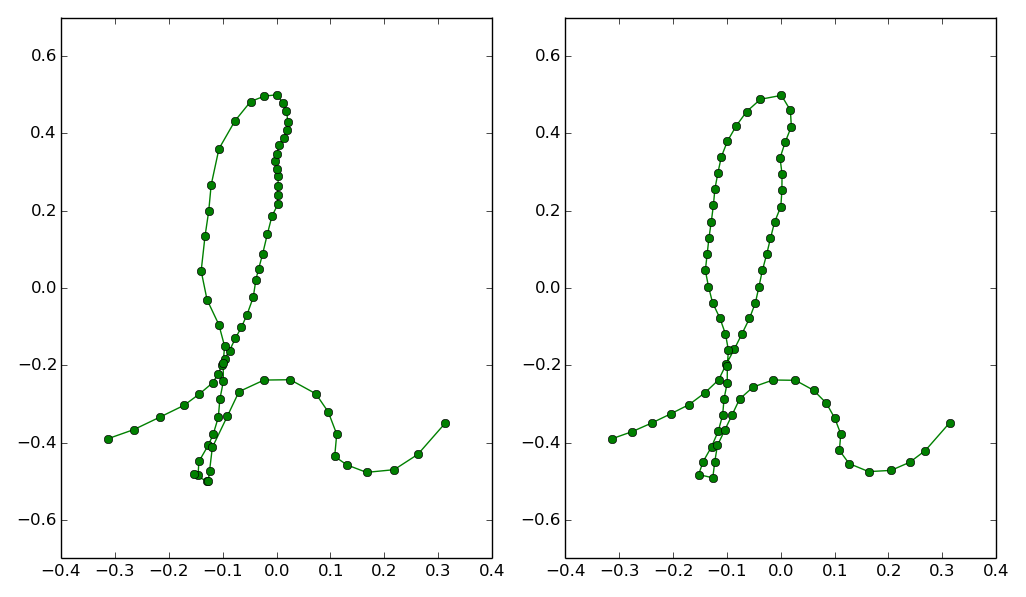
\includegraphics[width=0.9\textwidth]{figures/pointRedis.png}
        \caption{Before and after applying point redistribution}
        \label{fig:pointRedis}
\end{figure}
~
\begin{algorithm}[H]
 \scriptsize
 \While{$ i \leq numPointsShape $}{
   $ lengthShape = lengthShape + calcDist(points[i],points[i+1]) $\;
   $ scaleLength[i] = lengthShape $\;
   $ step = lengthShape / numPointsShape $\;
   $ j = 0 $\;
   \For{$ i= 0 \to numPointsShape-2 $}{
   		\While{$ i*step \geq scaleLength[j] $}{
   			$ j=j+1 $\;
   		}
   	$ j = j-1 $\;
    $ x0 = shape[j] $\;
    $ y0 = shape[j + numPointsShape] $\;
    $ x1 = shape[j + 1] $\;
    $ y1 = shape[j + 1 + numPointsShape] $\;
    $ diff = i*step - scaleLength[j] $\;
    $ dist = scaleLength[j + 1] - scaleLength[j] $\;
    $ newShapeX = x0 + diff*(x1-x0)/dist$\;
    $ newShapeY = y0 + diff*(y1-y0)/dist$\;
    }
  }
  \caption{Point uniformization algorithm}
  \label{al:points}
\end{algorithm}
\vspace{1cm}
By the use of this technique, we expect a better result in the decomposition of the shape in its eigenvectors and eigenvalues and thus, a more reliable correctness assessment using distance metrics in the eigenspace. Once the preprocessing is done, the demonstration shapes can be projected to the correspondent eigenspace obtaining a result similar to the one shown in figure \ref{fig:eigenspaces}. The shapes projected are shown in figure \ref{fig:shapeList}

\begin{figure}[h!]
        \centering
        \begin{subfigure}{0.4\textwidth}
                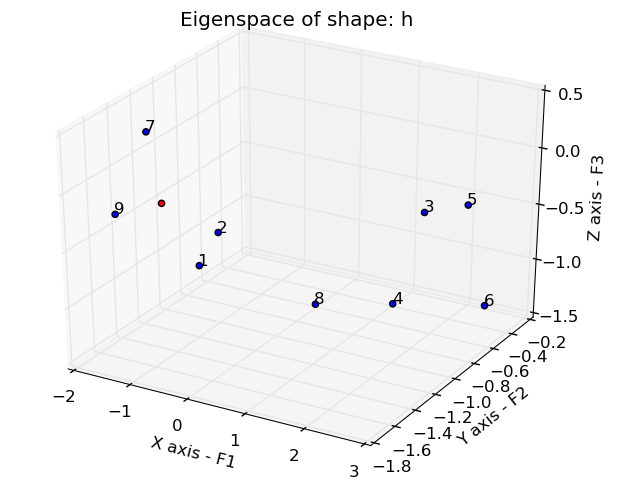
\includegraphics[width=1\textwidth]{figures/eigenBefore.png}
                \caption{Before}
                \label{fig:eigenBefore}
        \end{subfigure}
        \begin{subfigure}{0.4\textwidth}
                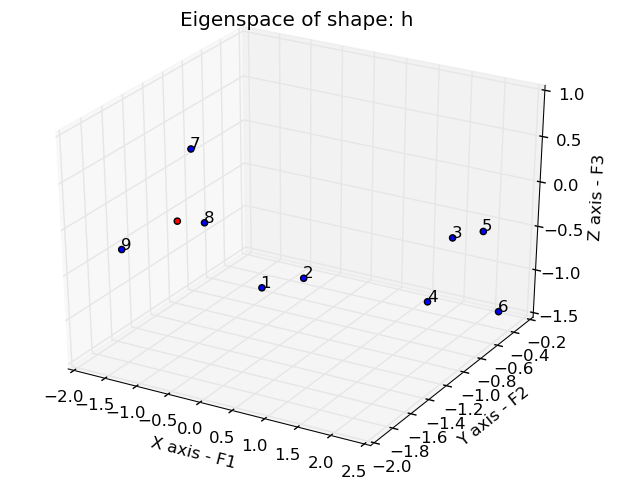
\includegraphics[width=1\textwidth]{figures/eigenAfter.png}
                \caption{After}
                \label{fig:eigenAfter}
        \end{subfigure}
        \caption{Demonstration shapes projected to the eigenspace with and without point uniformization (blue), and the reference shape (red).}
        \label{fig:eigenspaces}
\end{figure}


\begin{figure}[h!]
        \centering
        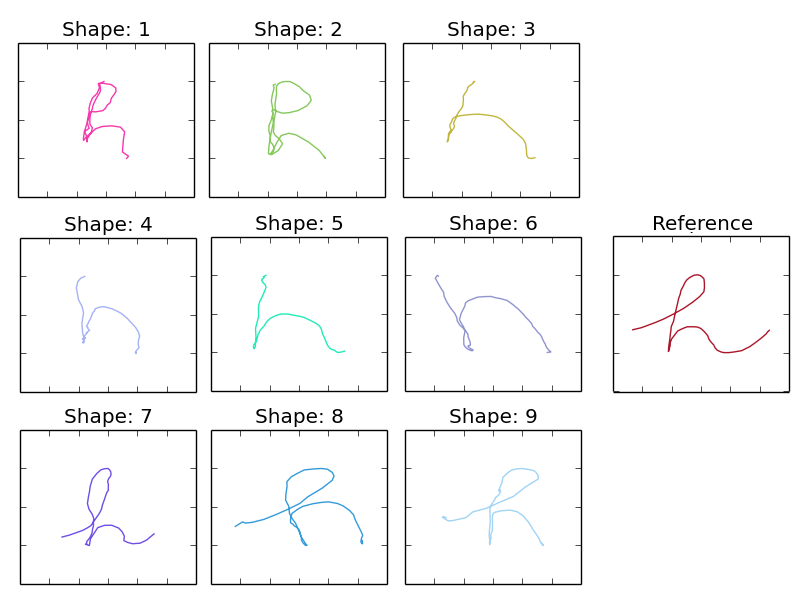
\includegraphics[width=0.7\textwidth]{figures/shapeList.png}
        \caption{List of shapes projected to the eigenspace}
        \label{fig:shapeList}
\end{figure}

We can observe how in figure \ref{fig:eigenAfter}, the preprocessing applied allows a correspondence between the qualitative and the quantitative assessment, locating shapes 7,8 and 9 together and closer to the reference one. Shapes 1 and 2 are located a bit farer since the samples show repeated strokes and finally, the different writing style shapes (3,4,5 and 6) are located far away from the reference.

However, choosing the appropriate metric and dataset to compose the eigenspace and project the shapes by itself does not assure a better distance assessment and thus a visual correctness correspondence shape-distance. At this point, it is necessary to know, first, if the types of shapes can be classified, and if it is possible, which clustering method would be more reliable for this task.


\section{Rating shapes using distance}
In order to rate the shapes provided by the user quantitatively and be consistent in the qualitative visual assessment, it has been necessary to test several methodologies; K-means using different distance metrics and SVM clustering method.
 
\subsection{Shape distance metrics in the eigenspace}  

In \cite{moon2001computational}, Moon and Phillips look at the effect of four traditional distance measures in the context of face recognition: City-block (L1 norm), squared Euclidean distance (L2 norm), angle, and Mahalanobis distance. 

\textbf{L1} City Block Distance
\begin{equation}
        d(x,y) = |x-y| = \sum_{i=1}^{k}|x_i - y_i|
\end{equation}

\textbf{L2} Euclidean Distance (Squared)
\begin{equation}
        d(x,y) = ||x-y||^2 = \sum_{i=1}^{k}(x_i - y_i)^2
\end{equation}

\textbf{Angle} Negative Angle Between Image Vectors
\begin{equation}
        d(x,y) = - \frac{x\cdot y}{\Arrowvert x\Arrowvert \Arrowvert y\Arrowvert} = -\frac{\sum_{i=1}^{k}(x_i - y_i)}{\sqrt{\sum_{i=1}^{k}(x_i)^2{\sum_{i=1}^{k}(y_i)^2}}}
\end{equation}	

\textbf{Mahalanobis} Mahalanobis distance
\begin{equation}
        d(x,y) = - \sum_{i=1}^{k} \frac{1}{\sqrt{\lambda_i}}x_iy_i
\end{equation}

Where $\lambda_i$ is the \textit{i}th Eigenvalue corresponding to the \textit{i}th Eigenvector. This is a simplification of Moon's definition:

\begin{equation}\label{eq:moore}
        d(x,y) = - \sum_{i=1}^{k} z_ix_iy_i \quad \textrm{where} \quad z_i = \sqrt{\frac{\lambda_i}{\lambda_i + \alpha^2}} \backsimeq \frac{1}{\sqrt{\lambda_i}} \quad \textrm{and} \quad \alpha=0.25
\end{equation}

Our experiments with the original formula showed poor results, hence our adoption of the definition in equation \ref{eq:moore}. Such experiments are summarized in table \ref{tab:distances} where K-means clustering method was used with different distance metrics.

\begin{table}[h!]
\centering
\begin{tabular}{l|l|l|l|l}
 		 		  & L1    & L2 & Angle & Mah \\ \hline	
Performance  	  & 77\% &  72\%  &	70\%   &  74\% 	    	

\end{tabular}
\caption{Distance metric performance for classification using K-means.}
\end{table}\label{tab:distances}

In this context K-means with L1 City block distance shown the best accuracy. Note that these results correspond to a test performed using 20 random samples of the same type of shape that were not previously used to compose the eigenspace. To conclude, we can consider the possibility, by performing K-means using City block distance, a simple metric for an automatized assessment of letter correctness if we assume there is only one cluster with reasonable good shapes.

\subsection{Shape classification}
In figure \ref{fig:shapeList}, three different types of shapes can be visualized with a certain correspondence in the eigenspace. In order to automatically classify the shapes, different clustering algorithms can be tested to check which one can provide better cluster segmentation based on the type of letter. For that, two common clustering algorithms were used: K-means using L1 distance since shows the best performance in table \ref{tab:distances} and Support Vector Machines (SVM).

The results summarized in table \ref{tab:clustering} were acquired using 34 shapes of 3 different letters from the same subject obtained along several experiments. There, we can see how SVM performs better in terms of classification.


\begin{table}[h!]
\centering
\begin{tabular}{l|l|l}
 		 		  & \textbf{K-means + L1}  & \textbf{SVM}	\\ \hline	
 \textit{h}-9 samples  	  &   100\% 	      &    100\% 	    \\ \hline
 \textit{a}-11 samples    &   81.8\%  	      &    90.9\%		\\ \hline
 \textit{g}-14 samples	  &   71.4\% 	      &    92.9\% 	     	

\end{tabular}
\caption{K-means - SVM classification performance comparison.}
\end{table}\label{tab:clustering}


\subsection{Additional outcomes}
As a secondary outcome of this chapter, a ROS Android app able to show the user shape progression across all repetitions was developed (see figure \ref{fig:plotApp}). It allows to provide a quantitative assessment of the user progression after each repetition in real time.

\begin{figure}[h!]
        \centering
        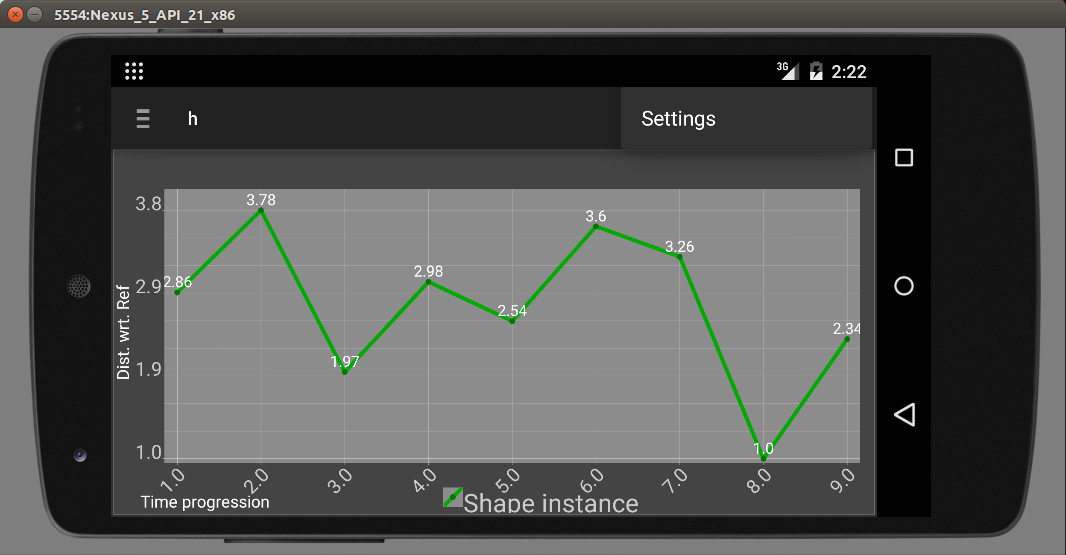
\includegraphics[width=0.8\textwidth]{figures/plotApp.png}
        \caption{ROS node App screenshot from Android Simulator that can be used to assess the user's  progression}
        \label{fig:plotApp}
\end{figure}

